\documentclass{article}
\usepackage[utf8]{inputenc}
\usepackage{float}
\usepackage{graphicx}
\usepackage[english]{babel}
\usepackage[margin=1.7in]{geometry}
\bibliographystyle{unsrt}
\usepackage{hyperref}
\usepackage{amsmath}
\usepackage{amssymb}
\usepackage{subcaption}
\usepackage{mathtools}


\begin{document}
\begin{titlepage}
	
	
	\title{Project 2 \\ Course 02445 \\ Project in Statistical evaluation of \\ artificial intelligence }
	\author{Rasmus J. P. s164564 \\ Nikolaj S. P. s183930}
	\date{January 2020}
	\maketitle
	
\subsection*{Summary}
Data science is a growing industry and has been since it's invention, many mathematical methods has come to life because of the drive to use data in every single industry. Data collection though can be expensive and time consuming so how do we decide what to collect and how to collect it? That is the job of a data scientist to answer and in this report we  examine different techniques of measuring bio-available phosphorous in soil and analyze them individually as well as determine whether the amount of bio-available phosporous influence the yield of a barley. \\ We fid that the yield certainly correlates with bio-available phosphprous but only up to a point whereas afterwards increasing the amount of phoshorous does not have a significant effect on the yield of barley. We conclude that the two measuring techniques were significantly different and make recommendation towards the more expensive technique.
	
\end{titlepage}


\section{introduction}
Crops need nutrients and if the levels of certain nutrients is too low the yield will be affected. Measuring the bio-available phoshporous BAP in soil is an important task for farmers in order to provide his or hers crops with sufficient amounts of nutrients. We know that the BAP is an important nutrient for plants but how big exactly is this influence of BAP to the yield of barley if it's there at all? That is the first aim of this report - to analyze and determine whether there is a significant influence from BAP on the yield and try and determine a model to describes this proposed effect of BAP. We analyze the models proposed and evaluate them on their fit to actual data. \\ A new and more expensive measurement technique "DGT" is proposed to be better than the older "Olsen P" technique. Anyzing these two techniques are the second aim for this report and to determine if there's a significant difference between the two in order to make a detailed and guided recommendation for farmers. We will determine  ... missing information about statistic test used to choose between Olsen and DGT.




\section{Data}
An experiment was performed on nine different fields spread across Denmark and Norway and each field partitioned into 4 plots. The yield of barley was measured and soil samples were analyzed by the two measuring techniques "DGT" and "Olsen P".
The data contains 4 variables, three continuous and 1 categorical. The continuous variables are \textit{yield ($hkg/ha$), DGT ($\mu/L$), Olsen P ($mg/100g$)} and the categorical is a unique identifikation number for each of the nine fields.
Observations were collected one from each of the four plots in the nine fields resulting in 36 observation of 4 variables.
We decided to impute two missing datapoints with the mean of other plots from the same field. OBS BURDE VI IKKE BRUGE ALLE PLOTS THIL AT REGNE DENNE MEAN?.
Our reasoning behind imputing the data was firstly, the fields do not have a high variance of yield between the plots, which means replacing the missing values with the mean would likely not be too far off the real values.
Secondly, field 11 is an importent datapoint with the lowest BAP, and removing it might heavily impact our models. See appendix .... ??..
 
\begin{figure}[H]
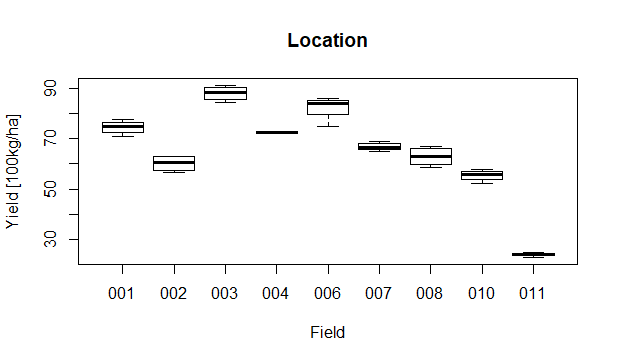
\includegraphics[width=\linewidth]{locationYield.png}
\caption{"Boxplot of yield for each field. We can see the variance within a field is relatively low, and location looks to have influence on yield"}
\label{fig:loc}
\end{figure}


Include a few good plots to highlight important features in data. You can put additional plots in the appendix.

\section{methods and analysis}

Describe the methods you used and why you decided to use them. 
Also discuss the assumptions behind the methods. Do not go into detail with theory.

\section{results}

Present the results.
Tables and figures are good ways of illustrating results.
What do your results show?
Discuss your results. How reliable are they?

\section{discussion and conclusion}

What are your conclusions? The conclusion should be connected to the aim of the report in the introduction.
	Highight important results
	
If you have found interesting problems/aspects that you haven’t carried out, you can specify them here as ‘future work’.

\end{document}